\section{Versuchsaufbau und Durchf"uhrung} % (fold)
\label{sec:durchf_uhrung}
	Im Voraus des Versuchs sollen mit Gleichungen \eqref{eqn:fourier} bis \eqref{eqn:b_n} die Fourierkoeffizienten einer Rechteck-, Dreieck und S"agezahnspannung berechnet werden.

	\subsection{Analyse}
	\label{subsec:analyse}
		Die drei Signale werden dann von einem Funktionsgenerator erzeugt und jeweils in einem Oszilloskop visualisiert.
		Das Oszilloskop ist dabei in der Lage, das Frequenzspektrum des Signals mit einer Fouriertransformation zu identifizieren.
		In diesem Spektrum kann das Verh"altnis der Fourierkoeffizienten zueinander bestimmt werden, um es mit den theoretisch bestimmten Werten der Koeffizienten zu vergleichen.

	\subsection{Synthese}
	\label{subsec:synthese}
		Im Folgenden Schritt wird ein Signalgenerator benutzt, der $\sin$- Funktionen der Frequenzen $\nu$, $2\nu$, bis $9\nu$ erzeugen und addieren kann.
		Zun"achst wird dabei jeden Amplitude der einzelnen Signale auf die entsprechenden Fourierkoeffizienten eingestellt.
		Dabei werden die Spannungsbetr"age der Funktionen f"ur $\mathrm{n} > 0$ relativ zur Eingangsspannung $U_0$ berechnet.

		\clearpage

		\begin{wrapfigure}{r}{6cm}
			\centering
			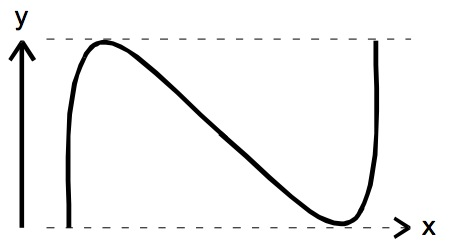
\includegraphics[width = 4cm]{img/lissajous.jpeg}
			\captionsetup{format=plain}
			\caption{Lissajous-Figur der 3. Oberwelle in Phase \cite{anleitung}.}
			\label{fig:lissajous}
		\end{wrapfigure}

		Anschlie"send wird die Phase $\varphi$ zwischen den Oberwellen und dem Hauptsignal justiert, sodass sie mit den Phasen der Fouriersummanden "ubereinstimmen.

		Daf"ur wird das Hauptsignal auf den X-Eingang und das Signal der Oberwelle auf den Y-Eingang des Oszilliskopes gelegt, wodurch dieses eine entsprechende Lissajous-Figur darstellt.
		Anhand dieser Figuren l"asst sich leicht erkennen, ob die Phase $\varphi$ zwischen den Signalen 0 oder $\pi$ betr"agt.
		Abbildung \ref{fig:lissajous} zeigt die Lissajous-Figur der dritten Oberwelle bei einer Phase $\varphi = 0$.

		Schlie"slich werden alle Signale summiert und wiederum auf dem Oszilloskop ausgegeben.
		Die Resultierende Funktion ist die Fouriersynthese der ersten neun Fourierkomponenten.

		\clearpage